%\RequirePackage{amsmath}
\documentclass[12pt]{article}

\usepackage{float}
\usepackage{multirow}
\newcommand{\ts}{\textsuperscript}
\usepackage{xcolor}
\usepackage{amssymb}
\definecolor{light-gray}{gray}{0.95}
\newcommand{\code}[1]{\colorbox{light-gray}{\texttt{#1}}}
\usepackage{graphicx}
\graphicspath{{plots/}}


\begin{document}



\title{
	%\logo{
%Computational Approach to School Geometry
	The Monte Carlo Method
%	}
}
\author{ Rahul Ramachandran% <-this % stops a space
}

\date{\vspace{-4ex}}

\maketitle


\section{Overview}

\subsection{General Overview}
The code uses the file 'inp.txt' as input, extracts the numbers $N$ and $K$ from the file, and distributes the task of generating $N$ random coordinates to 
$K$ threads to approximate the value of $\pi$ using the Monte Carlo Technique. It produces the file 'output.txt', which contains the computed approximate value
of $\pi$, the time taken for execution, and the various randomly generated points.

\subsection{Code Overview}
First, $K$ threads are created, and $N$ is distributed between the threads, to speed up the computation of random coordinates. The threads call the 
Monte Carlo function, which computes the random coordinates, and returns the number of points inside the unit circle. The total number of points generated inside the circle
is found by adding the number found by each thread, and dividing this result by the total number of points generated gives us $\frac{\pi}{4}$.



\section{Low Level Details}

\subsection{Global Variables}
The shared memory in this program comprises of the five global vectors:
\begin{itemize}
  \item \texttt{vector<ll> indices}: Each thread is assigned a thread number when it runs the Monte Carlo function. This vector is used to distribute
  the indices/thread-numbers to the threads. For instance, the first thread is assigned \texttt{indices[$0$]}, which is $0$. (\texttt{indices[$j$]} = $j$)
  \item \texttt{vector<ll> points\_inside\_circle}: This global vector contains the number of points found inside the circle per thread. For example, \texttt{points\_inside\_circle[$j$]} contains the 
  number of points found inside the circle by the $(j+1)^{th}$ thread.
  \item \texttt{divided\_npoints}: This global vector is used to divide the total number of points to be generated between the threads. For instance, if there are $4$ threads and $6$ points, the vector will contain \{$2,2,1,1$\}
  \item \texttt{vector< vector < pair <float, float> > > coordinates}: This is a vector of vectors, and is used to store all the coordinates. The $j^{th}$ vector contains the points for the $(j+1)^{th}$ thread.
  \item \texttt{vector< vector<int> > flag\_inside\_circle}: This is another vector of vectors, and is used to flag which coordinates are inside the unit circle and which aren't. For example, if the third value of the first vector in \texttt{flag\_inside\_circle} is $1$,
  then the third coordinate in the first vector of the global vector \texttt{coordinates} lies \emph{inside} the unit circle (This is the third coordinate generated by the first thread). Similarly, a zero implies that the point lies outside the unit circle.
\end{itemize}

\subsection{Monte Carlo Function}
The function takes the thread-number (or index) as input. It accesses everything else through this index and the global variables. A \emph{Mersenne RNG} is used to generate the random numbers. This is done '\texttt{divided\_npoints[index]}' number of times. The value of $x^2 + y^2$ is compared
with $1$ to check if the randomly generated points lie in the circle or not. If they do, the counter is incremented, and the appropriate flag is set. At the end of the function, the computed values are stored in the corresponding global variables before returning.

\subsection{Main Function}
\subsubsection{Initialization}
The file 'input.txt' is read, and the numbers $N$ and $K$ are extracted. The \emph{remainder} on dividing $N$ by $K$ is calculated.
To distribute $N$ numbers into $K$ buckets, we first distribute $\lfloor \frac{N}{K} \rfloor$ numbers to each bucket, and then give 1 number to the first
\emph{remainder} buckets. For example, if there are 50 numbers and 8 threads, the first rem(50/8) = 2 threads get $\lfloor \frac{50}{8} \rfloor + 1 = 7$ numbers, and
the other threads get $6$ numbers. Thus, the first 2 threads generate $7$ random coordinates, while the other threads generate $6$.
\subsubsection{Creating the threads}
A for loop is used to create the threads, which all run on the 'Monte Carlo' function. The argument passed to the function is a pointer to the index $i$ for the thread. The threads all execute the function,
and populate the vectors \texttt{points\_inside\_circle}, \texttt{coordinates} and \texttt{flag\_inside\_circle}. \texttt{pthread\_join} is then called, before control passes back to the main thread.


\subsubsection{Computing the value of $\pi$}
The entire procedure is based on the following: Given a square and an inscribed circle, the probability that a randomly chosen point lies inside the circle equals the ratio of the areas of the circle and the square,
assuming a uniform distribution. This comes out to be $\frac{\pi r^2}{4r^2} = \frac{\pi}{4}$. If many points are randomly chosen, the empirical probability closely approximates the actual probability, and equals the ratio of
the number of points observed inside the circle, and the total number of points. Thus, multiplying this ratio by 4 gives us an approximation for $\pi$. (Note that the ratio is invariant to scaling, and we can choose $r=1$ WLOG)

\noindent The main thread does exactly this. It uses the vector \texttt{points\_inside\_circle} to find the total number of points found inside the circle, divides by the total number of points to find the ratio, and multiplies this result by 4 to find an approximation
for $\pi$.


\subsubsection{Output}
The program generates the text-file 'output.txt' using the various global vectors

The file contains information in the following format: (for example) \\

\texttt{
\noindent Time: 50000 $\mu$s \\ \\
Value Computed: 3.14597 \\ \\
Log: \\ \\
Thread1: 125000, 98152\\
Points inside the square:(-0.860914,-0.296664), (-0.0881785,-0.902898), \dots \\
Points inside the circle:(-0.860914,-0.296664), (-0.0881785,-0.902898),  \dots \\ \\
Thread2: 125000, 98379\\
$\vdots$ \\
}
\section{Analysis}

\subsection{Time taken vs No. of threads}
The number of input points was fixed at $6 \cdot 10^6$. The number of threads was varied from $2$ to $32$ as $2, 4, 8, 16, 32$. The average value of time taken 
was computed over $5$ trials, and the plot below was obtained.


\begin{figure}[H]
  \centering
  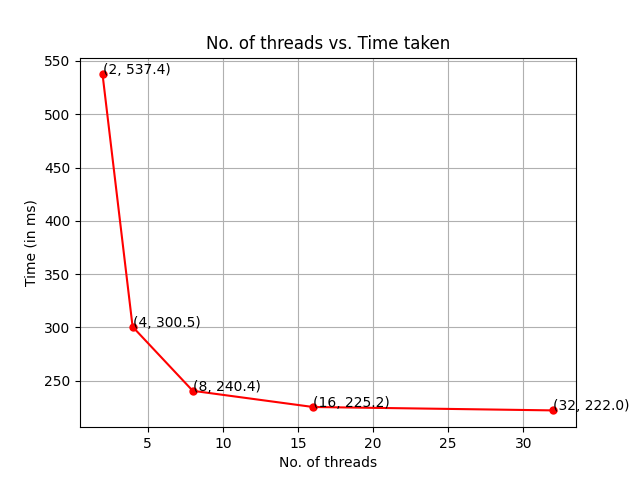
\includegraphics[width=\columnwidth]{Figure_1.png}
  \caption{No. of threads vs. Time taken}
  \label{fig-1}
  \end{figure}

  Clearly, the time taken decreases with the number of threads, but not proportionally; the increase in speedup slows down as the number of threads goes up. This happens for a few reasons:
  
  \begin{itemize}
    \item By Amdahl's Law, the speedup is $ <= \frac{1}{S+\frac{1-S}{N}}$, where $S$ is the fraction of serial code. In other words, as the nummber of threads increases, the serial portion of the code becomes the bottleneck, as the speedup will always be $<= \frac{1}{S}$
    \item Since there is an inherent limit to the multithreading capability of a system (by the number of cores), increasing the number of threads beyond a point will not help reduce the time taken.
    \item After a point, thread overheads (like context-switching between many threads for instance) become significant, and outweigh the speedup gained due to multithreading.
  \end{itemize}


% \subsection{Time Elapsed}
% The time elapsed for various values of $N$ and $K$ is tabulated below:


% \begin{table}[H]
%         \centering
%         \begin{tabular}{|c|c|c|c|}
%         \hline
%           K & N = 500,000 & N = 5,000,000 & N = 50,000,000\\ \hline

%           $1$ & 0.654 & 18.9 & 576.33\\ 
%              $4$ & 0.314 & 7.1 & 215.81\\ 
%            $16$ & 0.188 & 5.26 & 162.01\\ \hline
%         \end{tabular}
%         \caption{Time (in seconds) for various values of N as the number of child processes K is varied}
%         \label{tab:my-table}
%     \end{table}


% From the table, it is clear that there is a significant decrease in time elapsed as the number of child processes is increased.
% Note that beyond a point, the decrease is small, because the number of processes that can be executed parallely is limited for a given processor.


\subsection{Time taken vs Number of initial points}

\begin{figure}[H]
  \centering
  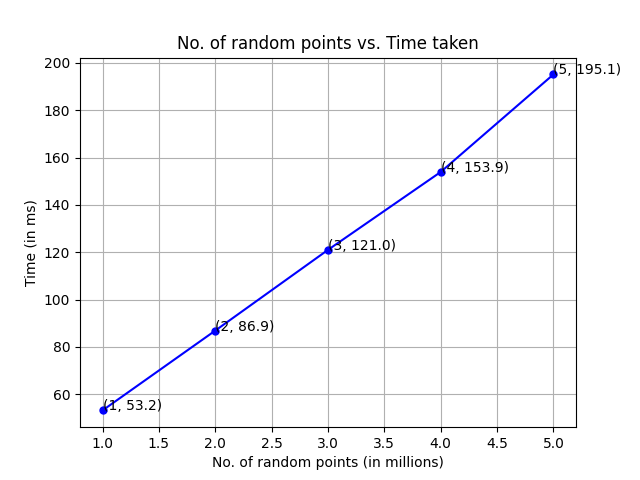
\includegraphics[width=\columnwidth]{Figure_2.png}
  \caption{No. of random points vs. Time taken}
  \label{fig-1}
  \end{figure}

  The number of threads was fixed at $32$. The number of points generated was varied from $1$ to $5$ million. The average value of time taken 
  was computed over $5$ trials, and the plot below was obtained. 

  Since the number of threads is fixed, assuming unit time cost for the generation of a random number, we would expect the time taken to generate all the points 
  to be proportional to $n$, or the complexity to be $O(n)$, since the main cost involved in the Monte Carlo process is the generation of random numbers. This is exactly what is observed 
  in the linear plot.

  \subsection{Accuracy in the value of $\pi$}
  The value of $\pi$ was measured for various number of randomly generated points:
  \begin{itemize}
    \item For \textbf{1000} points, the value of $\pi$ was \textbf{3.248}
    \item For \textbf{100000} points, the value of $\pi$ was \textbf{3.1348}
    \item For \textbf{1000000} points, the value of $\pi$ was \textbf{3.14212}
    \item For \textbf{1000000000} points, the value of $\pi$ was \textbf{3.14149}
  \end{itemize}

  The value approaches $3.14159$, but the convergence is extremely slow, because of the probabilistic randomness involved in the Monte Carlo process.
  

% \begin{table}[H]
%   \centering
%   \begin{tabular}{|c|c|c|c|}
%   \hline
%     N = 500,000 & N = 1,000,000 & N = 5,000,000 & N = 50,000,000\\ \hline

%      0.654 & 1.87 & 18.9 & 576.33\\ \hline
      
%   \end{tabular}
%   \caption{Time (in seconds) for various values of N for K = 1}
%   \label{tab:my-table-2}
% \end{table}



\end{document}